\documentclass{article}
\usepackage[utf8]{inputenc}
\usepackage[spanish]{babel}
\usepackage[shortlabels]{enumitem}
\usepackage{graphicx}
\usepackage{mathtools}
\usepackage{amsfonts}
\usepackage{minted}
\usepackage{hyperref}
\hypersetup{
    colorlinks=true,
    linkcolor=blue,
    urlcolor=cyan
  }

\title{Ejercicios de computación cuántica}
\author{Adrián Enríquez Ballester}
\date{\today}

\begin{document}
\maketitle

\subsection*{Ejercicio 1}

La puerta SWAP para 2 qubits se define como SWAP $|x\rangle|y\rangle
= |y\rangle|x\rangle$. Escribir la puerta SWAP como un circuito
cuántico que involucre solo puertas CNOT.

\subsubsection*{Respuesta}

El diagrama del circuito es 

\begin{center}
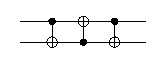
\includegraphics[scale=2.5]{swap-circuit.pdf}
\end{center}

que ha sido generado utilizando
\href{https://www.mathstat.dal.ca/~selinger/quipper/}{Quipper} con
el siguiente código:

\begin{minted}{haskell}
print_simple PDF $ do \(x, y) ->
  controlled_not_at y x
  controlled_not_at x y
  controlled_not y x
\end{minted}


Sean $|\varphi_1\rangle = a|0\rangle + b|1\rangle$
y $|\varphi_2\rangle = c|0\rangle + d|1\rangle$ dos qubits
arbitrarios, veamos cómo actúa el circuito sobre ellos. El resultado
de aplicar la primera puerta CNOT sería

\begin{align*}
  |\psi_\text{I}\rangle
    &=\mathcal{U}_\text{CNOT}|\varphi_1 \varphi_2\rangle \\
    &= \mathcal{U}_\text{CNOT}\Big(
      (a|0\rangle + b|1\rangle)
        \otimes(c|0\rangle + d|1\rangle)
      \Big) \\
    &= \mathcal{U}_\text{CNOT}\Big(
      a|0\rangle \otimes c|0\rangle
        + a|0\rangle \otimes d|1\rangle 
        + b|1\rangle \otimes c|0\rangle 
        + b|1\rangle \otimes d|1\rangle
      \Big) \\
    &= a|0\rangle \otimes c|0\rangle
        + a|0\rangle \otimes d|1\rangle 
        + b|1\rangle \otimes c|1\rangle 
        + b|1\rangle \otimes d|0\rangle
\end{align*}

A continuación, al estado anterior se le aplicaría otra puerta CNOT
pero con las entradas intercambiadas:

\begin{align*}
  |\psi_\text{II}\rangle
    &=\mathcal{U}_\text{CNOT}'|\psi_\text{I}\rangle \\
    &= \mathcal{U}_\text{CNOT}'\Big(
        a|0\rangle \otimes c|0\rangle
        + a|0\rangle \otimes d|1\rangle 
        + b|1\rangle \otimes c|1\rangle 
        + b|1\rangle \otimes d|0\rangle
      \Big) \\
    &= a|0\rangle \otimes c|0\rangle
        + a|1\rangle \otimes d|1\rangle 
        + b|0\rangle \otimes c|1\rangle 
        + b|1\rangle \otimes d|0\rangle
\end{align*}

Por último, se aplicaría de nuevo otra puerta CNOT:

\begin{align*}
  |\psi_\text{III}\rangle
    &=\mathcal{U}_\text{CNOT}|\psi_\text{II}\rangle \\
    &= \mathcal{U}_\text{CNOT}\Big(
        a|0\rangle \otimes c|0\rangle
        + a|1\rangle \otimes d|1\rangle 
        + b|0\rangle \otimes c|1\rangle 
        + b|1\rangle \otimes d|0\rangle
      \Big) \\
    &= a|0\rangle \otimes c|0\rangle
        + a|1\rangle \otimes d|0\rangle 
        + b|0\rangle \otimes c|1\rangle 
        + b|1\rangle \otimes d|1\rangle
\end{align*}

Teniendo en cuenta este resultado general, y que $|a|^2 + |b|^2 = 1$
y $|c|^2 + |d|^2 = 1$, la puerta actúa de la siguiente manera sobre
la base canónica:

\begin{align*}
  \mathcal{U}_\text{SWAP}|00\rangle &= |00\rangle 
    \;\;\;\;\;\;(a = 1, c = 1)\\
  \mathcal{U}_\text{SWAP}|01\rangle &= |10\rangle 
    \;\;\;\;\;\;(a = 1, c = 0)\\
  \mathcal{U}_\text{SWAP}|10\rangle &= |01\rangle 
    \;\;\;\;\;\;(a = 0, c = 1)\\
  \mathcal{U}_\text{SWAP}|11\rangle &= |11\rangle
    \;\;\;\;\;\;(a = 0, c = 0)\\
\end{align*}

\subsection*{Ejercicio 2}

Supongamos que queremos factorizar el número $M = 33$ con el
algoritmo de Shor.

\begin{enumerate}[(a)]
  \item ¿Qué valor elegimos para $m$, el número de qubits del primer
    registro?
  \item Supongamos que elegimos aleatoriamente $a = 2$. Calcular con
    el ordenador o una calculadora cuál es el período $r$ de $f(x)
    = a^x \text{ mod } M$.
  \item Supongamos que, tras realizar la QFT y medir, el resultado
    es $c = 614$. ¿Es este un $c$ de los que llamamos ``buenos''?
\end{enumerate}

\subsubsection*{Respuesta}

En este registro queremos poder codificar en binario el número $M^2
= 1089$. Como $2^{10} - 1 < 1089 < 2^{11} - 1$, elegiremos $11$
qubits.

En cuanto al período de $f$, vamos a utilizar
\href{http://downloads.haskell.org/~ghc/latest/docs/html/users_guide/ghci.html#using-ghci}{GHCi}
para calcular los primeros valores de la función:

\begin{minted}{haskell}
f x = 2 ^ x `mod` 33
take 40 . map f $ [0..]
\end{minted}


\begin{minted}{haskell}
[1,2,4,8,16,32,31,29,25,17,1,2,4,8,16,32,31,29,25,17,1,2,4,8,16,32,
31,29,25,17,1,2,4,8,16,32,31,29,25,17]
\end{minted}


Observando el resultado se puede apreciar un patrón de longitud $10$
que parece repetirse indefinidamente, por lo que vamos a considerar
que el período de $f$ es $r = 10$.

Por último, vamos a intentar encontrar un $j$ para el que $c$ cumple
la condición de ser ``bueno''. Empezamos a probar todos los números
naturales desde $0$:

\begin{minted}{haskell}
check j = abs (614 - j * ((2 ** 11) / 10)) <= 1 / 2
head . filter check $ [0..]
\end{minted}


\begin{minted}{haskell}
3
\end{minted}


Para $j = 3$ se cumple la condición, por lo que 614 es un ``c
bueno''.

\subsection*{Ejercicio 3}

Para un sistema de 3 qubits, escribir el estado
$\mathcal{U}_\text{QFT}|3\rangle$ como un producto tensorial de tres
estados de un qubit, cada uno de ellos de la forma
$\frac{1}{\sqrt{2}}(|0\rangle + e^{2\pi i z}|1\rangle)$ para ciertos
$z$.

\subsubsection*{Respuesta}

Por una parte, el estado tras aplicar la puerta QFT sería 

\begin{align*}
  \mathcal{U}_\text{QFT}|3\rangle 
  &= \frac{1}{\sqrt{2^3}} 
    \sum_{c=0}^{2^3 - 1} e^{2\pi i 3 c / 2^3} |c\rangle \\ 
  &= \frac{1}{2\sqrt{2}}\Big(
      |0\rangle 
      + e^{2\pi i 3/8}|1\rangle 
      + e^{2\pi i 6/8}|2\rangle 
      + e^{2\pi i 9/8}|3\rangle 
      + e^{2\pi i 12/8}|4\rangle \\
      &\;+ e^{2\pi i 15/8}|5\rangle 
      + e^{2\pi i 18/8}|6\rangle 
      + e^{2\pi i 21/8}|7\rangle 
    \Big)
\end{align*}

Por otra, este estado pretende ser expresado como 

\begin{align*}
  &\frac{1}{\sqrt{2}}(|0\rangle + e^{2\pi i z_1}|1\rangle)
    \otimes \frac{1}{\sqrt{2}}(|0\rangle + e^{2\pi i z_2}|1\rangle)
    \otimes \frac{1}{\sqrt{2}}(|0\rangle + e^{2\pi i z_3}|1\rangle)
    \\
  = &\frac{1}{\sqrt{2}^3}\Big(
      |000\rangle
      + e^{2\pi i z_3}|001\rangle 
      + e^{2\pi i z_2}|010\rangle 
      + e^{2\pi i z_2}e^{2\pi i z_3}|011\rangle 
      + e^{2\pi i z_1}|100\rangle \\ 
      &+ e^{2\pi i z_1}e^{2\pi i z_3}|101\rangle 
      + e^{2\pi i z_1}e^{2\pi i z_2}|110\rangle 
      + e^{2\pi i z_1}e^{2\pi i z_2}e^{2\pi i z_3}|111\rangle 
    \Big) 
\end{align*}

para ciertos $z_1, z_2$ y $z_3$. Si se considera que todos ellos son
números reales, los productos de la forma $e^{2\pi i x}e^{2\pi i y}$
equivalen a $e^{2\pi i (x + y)}$. Teniendo además en cuenta el
número en decimal representado por las etiquetas de los qubits, la
expresión anterior se puede reescribir como

\begin{align*}
  &\frac{1}{2\sqrt{2}}\Big(
      |0\rangle
      + e^{2\pi i z_3}|1\rangle 
      + e^{2\pi i z_2}|2\rangle 
      + e^{2\pi i (z_2 + z_3)}|3\rangle 
      + e^{2\pi i z_1}|4\rangle \\ 
      &+ e^{2\pi i (z_1 + z_3)}|5\rangle 
      + e^{2\pi i (z_1 + z_2)}|6\rangle 
      + e^{2\pi i (z_1 + z_2 + z_3)}|7\rangle 
    \Big) 
\end{align*}

Esta tiene la misma forma que el estado que queremos representar por
lo que, igualando las subexpresiones que involucran a los $z_i$,
obtenemos el conjunto de ecuaciones

\begin{align*}
  z_3 &= 3/8 \\
  z_2 &= 6/8 \\
  z_2 + z_3 &= 9/8 \\
  z_1 &= 12/8 \\
  z_1 + z_3 &= 15/8 \\
  z_1 + z_2 &= 18/8 \\
  z_1 + z_2 + z_3 &= 21/8 \\
\end{align*}

cuya solución es $z_1 = 3/2$, $z_2 = 3/4$ y $z_3 = 3/8$, dando lugar
a la siguiente expresión final:

\begin{align*}
  \mathcal{U}_\text{QFT}|3\rangle 
  &= \frac{1}{\sqrt{2}}(|0\rangle + e^{2\pi i 3/2}|1\rangle)
    \otimes \frac{1}{\sqrt{2}}(|0\rangle + e^{2\pi i 3/4}|1\rangle)
    \otimes \frac{1}{\sqrt{2}}(|0\rangle + e^{2\pi i 3/8}|1\rangle)
\end{align*}

\end{document}
